
% \begin{itemize}
%     \item Principle, example STAs
%     \item Influence on STA of E/I balance, output firing rate, reversal potentials
%     \item Use as connection test: shuffled spike trains and height of STA, p-values, and the `area-over-start' heuristic for E vs I classification.
%     \item Evaluation of a connection test: `ternary' classification, summary measures, AUROC
%     \item Performance of the simple STA-height test, for different N
%     \item Influence of window length
%     \item What about Vm imaging affects detection the most?
% \end{itemize}



As shown in \cref{fig:diagram_Connectivity-Activity}, our idea for connection inference rests on the causal link `presynaptic spike' → `postsynaptic voltage bump'. I.e. we want to know for which neuron pairs a spike in one is reliably followed by such a bump in the other. The problem is that these bumps (the postsynaptic potentials or PSPs) are minute, and are easily drowned out by (1) other PSPs, (2) postsynaptic spikes, and (3) voltage imaging noise.

So, as is often done in neuroscience, we take the \emph{average} over many instantiations, so as to hopefully find a signal in the noise. Specifically, we take spike-triggered averages, or \textbf{STA}s, of neurons' voltage traces. If there is a connection from a neuron `M' to a neuron `N', then an STA of neuron N's voltage imaging signal, based on neuron M's spikes, would hopefully show the PSP.

And indeed, when we construct a few such STAs, we do see something resembling a PSP bump: \cref{fig:example_STAs}. We also find that the higher the firing rate of the presynaptic neuron, the cleaner the PSP-like shape is. This is of course because there are more presynaptic spikes and thus more windows to average over, which decreases the noise on the result. Finally, we see that inhibitory inputs result in downwards bumps in their STA, and excitatory inputs in upwards bumps.

\begin{figure}
    \hspace*{-3em}
    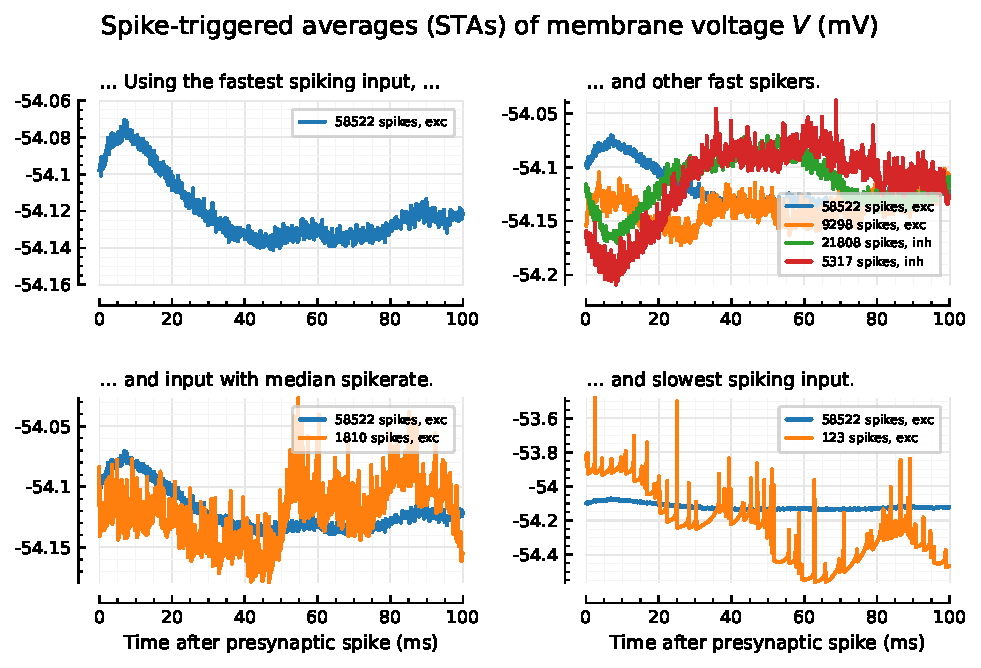
\includegraphics{example_STAs}
    \vspace*{1em}
    \captionn
        {Example STAs in the 10' simulation with 6500 inputs}
        {
        Note that every panel has a different y-axis (voltage) scale. The STA of the most active input is repeated in every panel (in faded blue), to allow a visual scale comparison nonetheless.\\
        The inset legends indicate with how many presynaptic spikes the STA was calculated, and whether the input was an excitatory or inhibitory one.\\
        The top right panel shows STAs of the 1\ts{st} and 100\ts{th} fastest spiking inputs, both within the excitatory inputs (\mpl{blue} shades), and within the inhibitory inputs (\mpl{orange} shades).\\
        Source: \nburl{2023-09-13__Clippin_and_Ceilin}.
        }
    \label{fig:example_STAs}
\end{figure}

Note that in this chapter -- and the next one -- we only look at the so called N-to-1 case (\cref{fig:diagram_Nto1}), where we simulate the voltage of one neuron, impinged on by N independent Poisson spiketrains. This is done for simplicity; it is only in the "Networks" chapter later on that we look at full networks, were inputs might be correlated with one another.

\begin{figure}
    \vspace*{2em}
    \hspace*{-1em}
    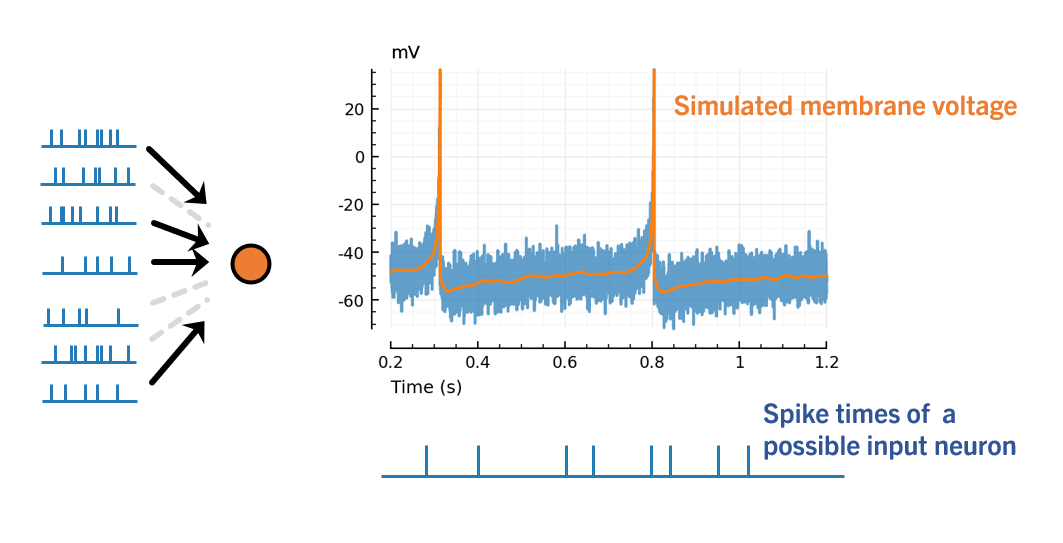
\includegraphics[w=1.2]{diagram_Nto1.png}
    \vspace*{-1.4em}
    \captionn
        {The `N-to-1' problem}
        {\Left: A neuron $N$ (orange circle), and the spike trains of other neurons in the network (blue). Some of these other neurons impinge directly on $N$ (black arrows), while others are not (directly) connected (dashed gray lines). Given only neuron $N$'s voltage signal and the other neurons' spiketrains, we want to detect the direct inputs, while rejecting the not-directly-connected spiketrains.\newline
        \Right: The simulated membrane voltage of the impinged-upon neuron (orange), and the same signal with Gaussian noise added, to simulate a voltage imaging signal (blue). Underneath the plot, one of the possible input spiketrains, time-aligned to the voltage signal.
        This alignment is used later to extract spike-triggered windows from the voltage signal.}
    \label{fig:diagram_Nto1}
\end{figure}

To use spike-triggered-averages as an actual connection test, we look specifically at the height of an STA, and compare it to a distribution of STA heights that we'd expect were the two neurons not connected. This is illustrated and explained in more detail in \cref{fig:STA-height-suffle}. This so called 'shuffle' test yields the proportion $p$ of how many shuffled (random) spiketrains yield an STA with a larger height than the real STA. In a following section (\nameref{sec:perf_quant}), we'll use this number (as $t = 1 - p$) to make predictions and compare them to the ground truth.

\begin{figure}
    \hspace{-5em}
    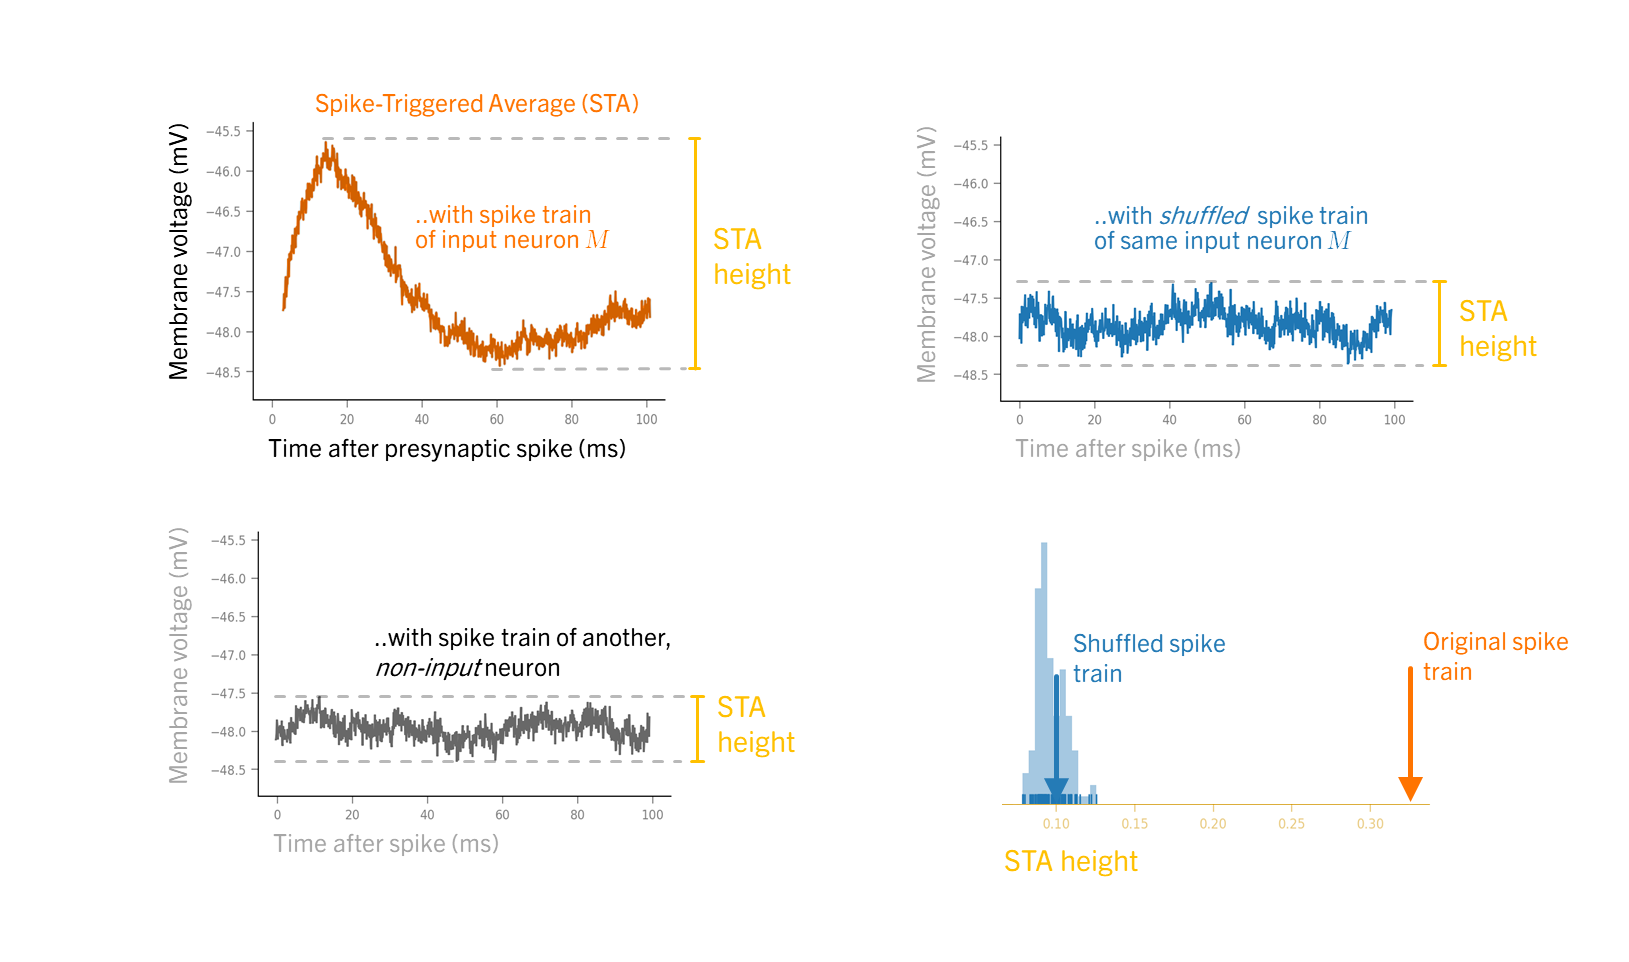
\includegraphics[w=1.7]{diagram_STA_test.png}
    \captionn
        {A simple connection test: STA height with shuffle control}
        {The spikes of a possible input neuron are aligned to the voltage trace of the neuron of interest $N$, as in \cref{fig:diagram_Nto1}. For every such spike, a 100-ms long window is cut out of the voltage of $N$. The average of all these windows is called the spike-triggered average (STA).\newline
        \Left: Two example STAs of neuron $N$'s membrane voltage: one for an actually connected input neuron, $M$ (top, orange); and one for a non-input neuron (below, gray).
        Given an STA signal $x$, we will use its height $h = \max(x) - \min(x)$ (also known as `peak-to-peak' or `ptp') to test whether two neurons are connected. \newline
        \Right: An STA of $N$'s membrane voltage using a shuffled version of $M$'s spike times (which is made by randomly permuting the inter-spike-intervals of $M$). This `shuffled STA height' provides a control for the STA height connection test statistic: "what do we expect the STA height to be if there is \emph{no} connection $M$→$N$".
        By calculating different such shuffles, we obtain a null-distribution for the STA height test statistic. And by comparing the real STA height to this distribution, we can calculate a $p$-value. Here, the real STA is larger than all shuffle controls, of which there are 100. So $p < 0.01$, and at α = 0.05, we conclude there is indeed a connection $M$→$N$.}
    \label{fig:STA-height-suffle}
\end{figure}



\FloatBarrier
\section{Ceiling and clipping}
\label{sec:ceil-n-clip}

\begin{figure}
    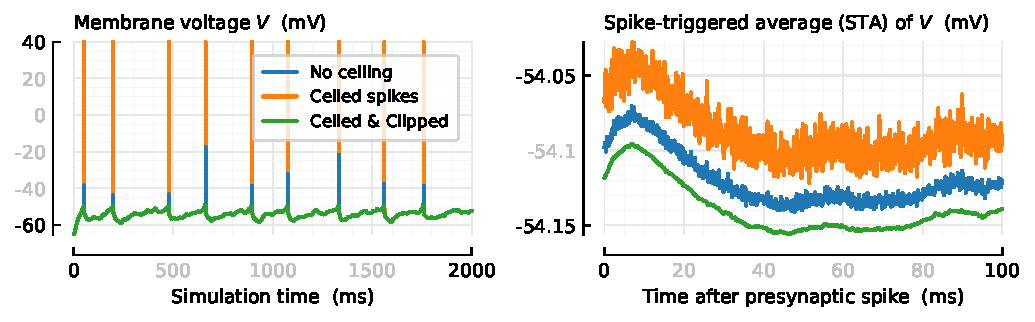
\includegraphics{ceil_n_clip__sigs_and_STAs}
    \caption
        {Example voltage traces and corresponding STAs, where the only difference is the height of spikes. In blue, the unmodified simulated voltage trace. In orange, the same, but with ceiled spikes (as in \cref{sec:spike_ceiling}). In green, the same as orange, but with the spikes clipped again after the ceiling (as explained in this section).\\
        Source: \nburl{2023-09-13__Clippin_and_Ceilin}.}
    \label{fig:ceil_n_clip__sigs_and_STAs}
\end{figure}

As explained in \cref{sec:spike_ceiling}, we modify our simulated voltage trace so that spikes have a consistent height. This modification has an effect on STAs, as is illustrated in \cref{fig:ceil_n_clip__sigs_and_STAs}: the blue trace is the signal without spike ceiling, the orange one with spike ceiling. Their corresponding STAs are shown on the right. Note that the orange STA (made with ceiled spikes) is much noisier than the blue STA (from the unmodified voltage trace).

This suggests a relatively easy intervention to drasticaly de-noise STAs, and presumably increase their effectiveness for network inference: namely to remove the spikes from the signal.

We tried this 'spike clipping' and it indeed drastically denoised the STA; see the green signal and STA in \cref{fig:ceil_n_clip__sigs_and_STAs}.
We show that this decreased noise in the STA does indeed lead to an increase in network inference performance, by running a connection detection test without and with this spike clipping. The results are shown in \cref{fig:ceil_n_clip_AUCs}: detection performance increases from an AUC of 0.56 for the non-clipped voltage trace, to an AUC of 0.79 for the voltage trace with clipped spikes.

\begin{figure}
    \begin{sidecaption}
        {
            Connection detection performance for the three ways of handling spikes shown in \cref{fig:ceil_n_clip__sigs_and_STAs}: not modifying them; ceiling them; and clipping them.
            The area-under-the-curve or AUC measure is explained in the next section.\\
            Source: \nburl{2023-09-13__Clippin_and_Ceilin}.
        }
        [fig:ceil_n_clip_AUCs]
        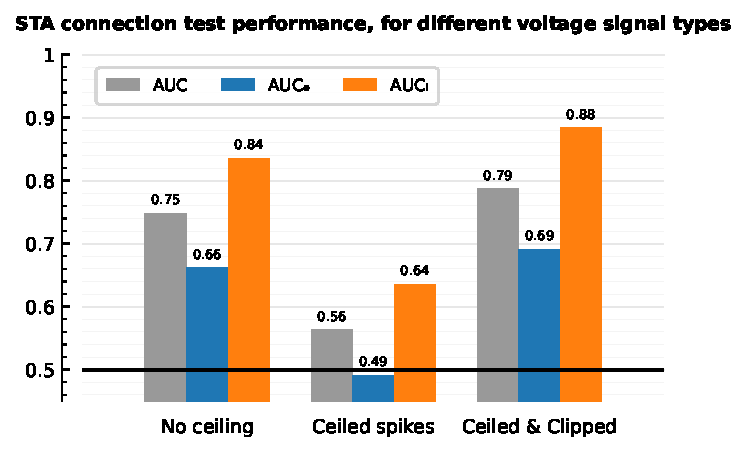
\includegraphics[w=1.03]{ceil_n_clip_AUCs}
    \end{sidecaption}
\end{figure}
% TODO: this graph is all wrong:
%   - The colours are confusing (should be organized the other way round: colours are sig type, grouping is exc/inh/both).
%   - The random chance line is much lower, as shown below.
%
% Where to edit this?
% can redo in new nb :)


\section{Window length}





\FloatBarrier
\section{Performance quantification}
\label{sec:perf_quant}

It is not easy to express in a single number how good a network inference algorithm is. Depending on what you find important as a user, different measures make more sense than others. This section looks at some measures to quantify the performance of our algorithms, and discusses the merits and disadvantages of each.

All the algorithms that we look at in this and the following chapter eventually output a single number per tested neuron pair (A, B): "How strongly do I believe there is a connection A→B?". (And: "Is that connection excitatory or inhibitory?": the sign of the number). We will call this connected-ness number "$t$".

To get actual predictions out of the algorithm,
% ("excitatory connection", "inhibitory connection", "unconnected")
we must apply a threshold $θ$ to these measures. If $|t| > θ$, we classify the pair as connected, and as unconnected otherwise. For the detected pairs, we classify them as excitatory if $t$ is positive, and inhibitory if it is negative.

Note that we use the same threshold for both excitatory and inhibitory connections. We could in fact use a different threshold -- and we briefly look at this in \cref{fig:perfmeasures_threshold_PPVs_EI} -- but for simplicity, we apply the same threshold for both types of connection.

Each threshold chosen yields a different tradeoff between recall and precision (\cref{fig:perfmeasures_θ_TPR_ROC}). At low thresholds, we can detect more connections ("true positives"); but we will also detect more non-inputs as being connected (false positives). This also lowers our precision.\\
Some definitions:
\begin{itemize}
    \item True positive rate (TPR), aka recall, sensitivity, and power: out of all true connections tested, how many did we correctly classify?
    \item False positive rate (FPR): out of all distractors we added to our test (randomly generated spiketrains), how many did we wrongly classify as an actual input?
    \item Precision, aka positive predictive value (PPV): out of all the neuron pairs that we classified as connected, how many are actually connected?
\end{itemize}

There are more measures that quantify the performance of a binary classifier at a given threshold than those three (such as negative predictive value, false discovery rate, false omission rate, ...).\footnotemark{}
But recall, FPR, and precision are commonly used ones.
\footnotetext{We do not actually perform binary classification: there are three classes (excitatory, inhibitory, unconnected). But it is not pure ternary (multiclass) classification either: we first classify as connected or not, and then (for the connected ones only), as excitatory or inhibitory. We could thus call it some kind of nested binary classification.}

\begin{figure}
    \includegraphics{perfmeasures_θ_TPR_ROC}
    \caption
    {Lower detection thresholds increase both true and false positives. On the right, true positive rates are plotted against the false positive rate, to obtain the so called receiver operating characteric or ROC curve. As the FPR increases more or less linearly with the decrasing detection threshold, both graphs look very similar.
    Source: \nburl{2023-09-13__Clippin_and_Ceilin}.}
    \label{fig:perfmeasures_θ_TPR_ROC}
\end{figure}

Note that true positive rate (TPR) and precision are similar, in that they both count correct classifications. (They both have the number of true positives in their numerator). But recall (TPR) looks at the number of true positives from the point of view of the ground truth (how many did we find), and precision looks at it from the perspective of the experimenter (out of what this algorithm gives us, how much is correct?).

False positive rate and precision are also similar, in that they both measure the number of false positives.\
One advantage of using FPR over precision though, is that FPR does not depend on the number of distractors (unconnected spiketrains) that we add to our tests.\footnote{Besides that, the more distractors we test, the more accurate our estimate of the FPR will be.}
Whereas we can arbitrarily increase precision by including less unconnected trains in our test -- up to the limit of 100\% precision, when we do not add any distractors and all tested trains are actually connected.

In our tests, we choose the number of unconnected trains rather arbitrarily. (For example, when we test 100 excitatory and 100 inhibitory inputs, we also generate and test 100 unconnected spiketrains). A better way to choose this number of distractors might be to estimate what a realistic fraction of unconnected neurons would be in a typical voltage imaging experiment. Given some patch of brain tissue and one of the neurons in it, how many of the other recorded neurons in that patch will be connected to it? This is an interesting research question -- and it is likely that answers can be found in the literature -- but we do not explore it here.

In \cref{fig:perfmeasures_θ_TPR_ROC}, we have looked at TPR and FPR, both as a function of the detection threshold and as a function of each other. In \cref{fig:perfmeasures_Fscores,fig:PR_curves_iso_Fβ,fig:perfmeasures_PR_curves_EI}, we look at TPR (recall) and precision, again as a function of the detection threshold and as a function of each other.

Because recall and precision both increase for 'better' detectors, we might combine them into one measure. This is what the $F$-scores do: they are the harmonic mean of recall and precision, with recall and precision weighted differently depending on a parameter $β$. The $F_β$ score attaches $β$ times as much weight to precision $P$ as to recall $R$:
\begin{equation}
    F_β = \frac{(1+β^2) · P · R}{β^2 · P + R}
\end{equation}
For $β = 1$, precision and recall are weighted equally. The $F_1$-score is also the most widely used of the $F$-scores.

% \rule[0.5ex]{4.5in}{0.55pt}

\begin{figure}
    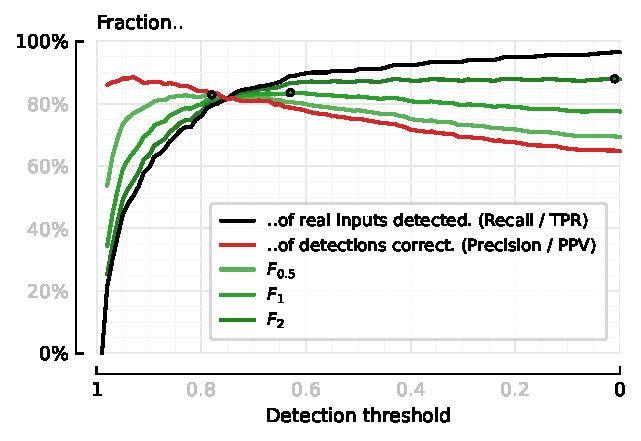
\includegraphics{perfmeasures_Fscores}
    \captionn
        {Lower detection thresholds trade-off higher recall for lower precision}
        {The $F_β$ scores interpolate between the two measures. $F_{→∞}$ is recall, $F_{→0}$ is precision. The black circles on the $F$-curves indicate their maxima. Different trade-offs between precision and recall (different $β$-values) thus dictate different optimal detection thresholds.}
    \label{fig:perfmeasures_Fscores}
\end{figure}

When we plot recall against precision, we get the so called PR-curves, shown in \cref{fig:PR_curves_iso_Fβ} for both excitatory and inhibitory inputs together, and in \cref{fig:perfmeasures_PR_curves_EI} for both types separately.
% Different $F_β$-scores (for the same $β$-value) correspond to the same rational function but with different offsetts. Different $β$-values on the other hand correspond to different scalings of the rational function.


\begin{figure}
    \begin{sidecaption}
        {Precision plotted against recall for the STA-test in the N=6500 inputs, 10-minute-recording experiment. Black dots indicate where three different $F_β$-scores reach their respective maximum values.}
        [fig:PR_curves_iso_Fβ]
        \includegraphics[w=0.88]{PR_curves_iso_Fβ}
    \end{sidecaption}
\end{figure}

\begin{figure}
    \begin{sidecaption}
        {Same as in \cref{fig:PR_curves_iso_Fβ}, but with excitatory and inhibitory inputs analysed separately. Note that we can detect more inhibitory inputs than excitatory inputs for the same precision value (or for the same false positive rate, as shown in \cref{fig:perfmeasures_θ_TPR_ROC}).}
        [fig:perfmeasures_PR_curves_EI]
        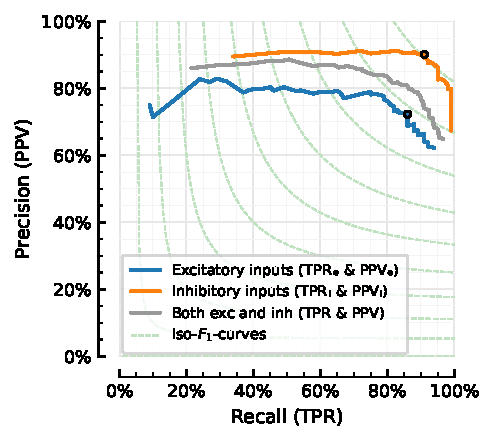
\includegraphics[w=0.88]{perfmeasures_PR_curves_EI}
    \end{sidecaption}
\end{figure}

\begin{figure}
    \begin{sidecaption}
        {\textbf{Excitatory and inhibitory inputs reach \maxF at different thresholds}.\\
        But for simplicity, whenever we use \maxF to evaluate a classifier, we will use only one threshold for both types of inputs, which will be a compromise between these two thresholds.}
        [fig:perfmeasures_threshold_PPVs_EI]
        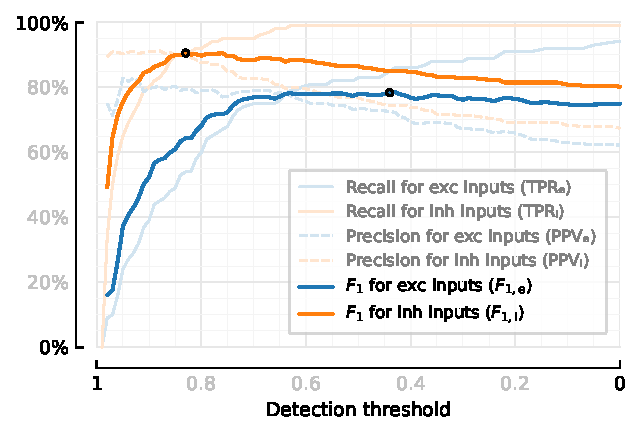
\includegraphics{perfmeasures_threshold_PPVs_EI}
    \end{sidecaption}
\end{figure}

Different thresholds yield different $F_β$-scores; but there is one threshold where your chosen $F$-score is maximal. This \maxF-score is a good candidate for the single "how good is this detector" measure we were looking for. We specifically choose $F_1$ as it weighs precision and recall equally (and we have no a-priori reason to prefer any one over the other), and because it is the most frequently used.

Another common single measure to quantify a classifier's performance is the area under its ROC-curve, or AUC, already shown in \cref{fig:perfmeasures_θ_TPR_ROC}. A disadvantage of the AUC is that it is less interpretable as a number than the \maxF score (which immediately gives a rough idea of how many true connections you'll detect, and how many of your detections are correct).
A disadvantage of the \maxF score is that it uses the precision, which, as discussed above, is rather arbitrary in our setup. AUC does not suffer this problem: the FPR is independent of how many distractors are added to the test.

To make the AUC scores somewhat more interpretable, we compare them to the AUC of a random classifier: a detector that classifies possible connections randomly. For simple binary classification, this results in an AUC of 0.5. But because we have three classes (unconnected, excitatory, and inhibitory), the random AUC will be lower. We simulated such random classifiers to find the chance-level AUC (\cref{fig:AUC_chance_level}), which turns out to be about $0.252$.

\begin{figure}
    \begin{sidecaption}
        {\textbf{Randomly classifying connections yields a chance level AUC $< 0.5$}.\\
        300 random test results, and their performance as connection detector, quantified as area under their ROC curves. Solid black line is the mean, dashed line is the median.\\
        In every of the 300 simulations, every connection (100 exc, 100 inh, and 100 unconnecteds) was assigned a random `t-value' uniformly between $-1$ and $1$; and then the classification threshold was swept over these t-values.\\
        Source: \nburl{2023-09-20__STA_conntest_for_diff_recording_quality_n_durations}.}
        [fig:AUC_chance_level]
        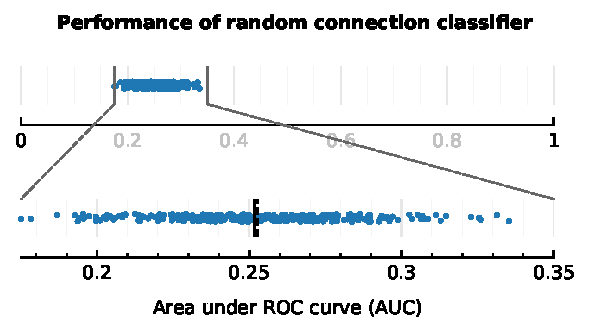
\includegraphics{AUC_chance_level}
    \end{sidecaption}
\end{figure}



\FloatBarrier
\section{Recording duration \& noise}

In this section we look at how longer or less noisy voltage imaging recordings improve connection inference. In \cref{fig:STA_perf_diff_snr}, the signal-to-noise ratio (SNR) is varied, and in \cref{fig:STA_perf_diff_rec_duration}, we vary the recording duration.

As might be expected, noisier and/or shorter recordings decrease detection performance, down to chance level in the limit (namely: for noise levels almost as high as the spikes; and for recordings shorter than a minute). As to recording duration, interestingly, we do not yet see any flattening off of the detection performance curve for longer recording duratoins, up to the durations that we simulated (up to 1 hour).

\begin{figure}
    \begin{sidecaption}
        {\textbf{Performance drops to chance level for noisier signals}.\\
        All simulations were 10 minutes long.
        Signal-to-noise (SNR) values on the x-axis are approximately (but not exactly) log-spaced. An SNR of `$\infty$' corresponds to no noise (i.e. the voltage signal straight out of the simulation, without any noise added).
        For every SNR value, five different simulations were run (gray dots), each with a different RNG seed for input firing rate and spiketrain generation. The mean performances of these five simulations are plotted with larger dots and are line-connected.
        Only the 100 highest-firing excitatory and inhibitory inputs were tested. An additional 100 unconnected spiketrains were generated and tested, with similar firing rates as those 200 high-firing real inputs.\\
        AUC chance level determined as in \cref{fig:AUC_chance_level}.\\
        Source: \nburl{2023-09-20__STA_conntest_for_diff_recording_quality_n_durations}.}
        [fig:STA_perf_diff_snr]
        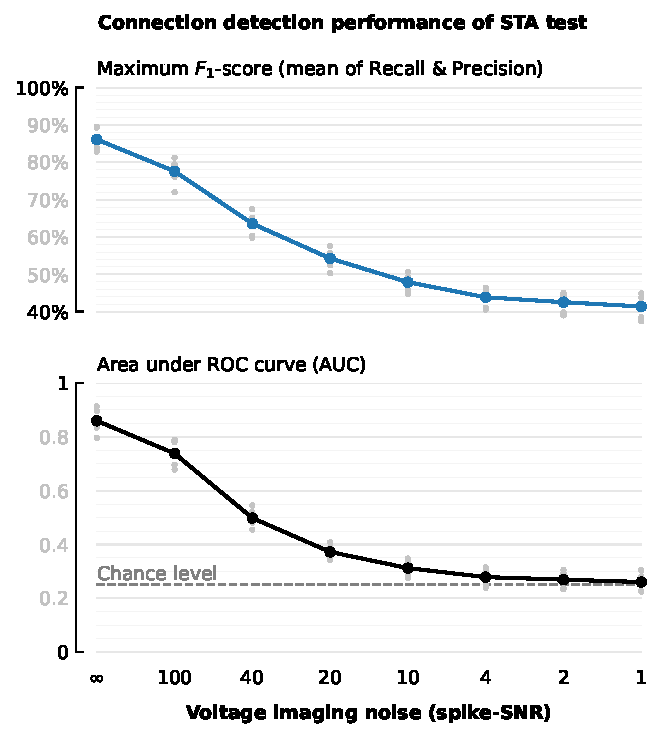
\includegraphics{STA_perf_diff_snr}
    \end{sidecaption}
\end{figure}

\begin{figure}
    \begin{sidecaption}
        {\textbf{Longer recordings allow more accurate connection inference}.\\
        All simulations had a voltage imaging noise level (spike-SNR) of 40.\\
        The simulation (`recording') durations are on a logarithmic axis. (The first two data points are at 10 and 30 seconds; the last one is at 1 hour). \\
        For more, see \cref{fig:STA_perf_diff_snr}'s caption.}
        [fig:STA_perf_diff_rec_duration]
        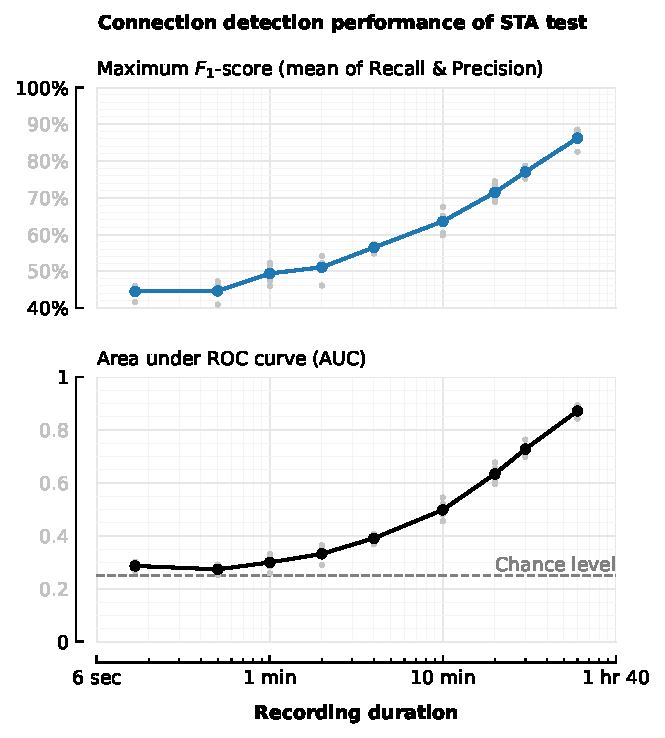
\includegraphics{STA_perf_diff_rec_duration}
    \end{sidecaption}
\end{figure}

For a concrete example of what a neuroscientist might expect from the STA-based connection test, we find that for a 10-minute recording with an SNR of 40 (which are more or less realistic for voltage imaging), the maximum $F_1$-score -- for the 200-highest firing inputs, and an additionally tested 100 unconnected spiketrains -- is about 65\%.

I.e, in the N-to-1 setup with 6500 inputs, for the 200 highest-firing of those inputs, we detect approximately 130 of them as being connected (±65\% recall). And of the spiketrains that we detect as inputs, about 65\% are correctly classified  (±65\% precision). I.e. 35\% of them are either excitatory connections classified as inhibitory and vice-versa; or they are random unconnected spiketrains classified as real inputs.

The area under the TPR/FPR-curve (AUC) for this recording duration and quality is about 0.50 (compared to the chance level of 0.25 -- see \cref{fig:AUC_chance_level}).



\section{EI balance}

In the rest of this thesis, we choose to have a fixed EI-balance (4:1 excitatory to inhibitory neurons, with  inhibitory neurons 4× stronger) and fixed excitatory and inhibitory reversal potentials. In this section however, we investigate these parameters, and wonder whether changing them has any effect on network inference performance.

\marginpar{
    \hspace*{-1.2em}
    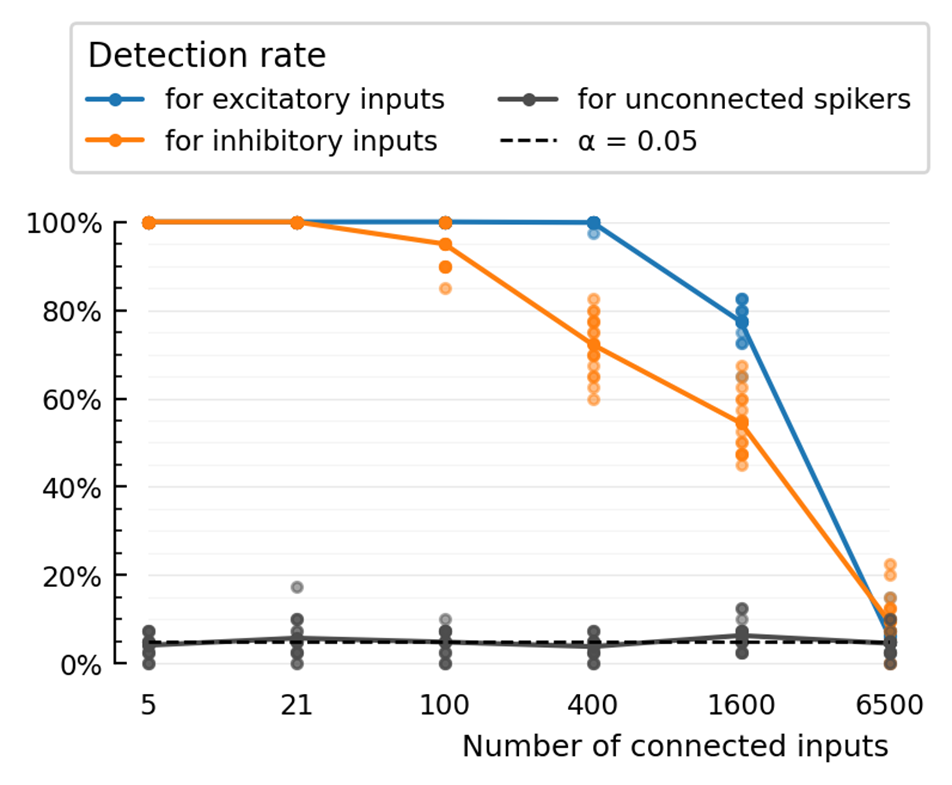
\includegraphics[w=1.2]{Nto1-high-N}
    \captionof{figure}{
        \textbf{STA performance for different $N$.}\\
        10-minute 4:1 EI-balanced simulations using the Izhikevich neuron. 16 simulations per condition, for different random number generator seeds.
        Source: \nburl{2022-05-02__STA_mean_vs_peak-to-peak}.
    }
    \label{fig:Nto1-high-N}
}

\underline{Note:} The results in this section were obtained before we switched to using an AdEx neuron model. They still use the Izhikevich neuron model (but with comparable parameters -- which were calculated using the correspondences found in \cref{sec:izh}). Second, in the rest of this chapter, we use a high number $N$ of input spiketrains (6500 in total). In this section however, we use just 27 input spiketrains.\footnote{
    Part of the reason for this initially lower number of spiketrains is that we still used our simulator written in Python and Numba here, which was slower than our later Julia simulator. We also still connection-tested \emph{all} inputs, and not just the highest firing (or a random subset). This made iterating with high $N$ prohibitively slow.
}
As might be expected, using a lower number of inputs makes connection inference much easier, as can be seen in \cref{fig:Nto1-high-N} (note that here, we test \emph{all} input spiketrains, and not just the highest firing ones as before. This gives a lower overall performance).

In the first subsection below, inhibitory and excitatory connections are equally strong ($Δg_\exc = \ Δg_\inh$). In the second subsection, the strength of inhibitory connections is varied.

\newcommand*{\sym}[1]{\ensuremath{#1}\xspace}  % used for definitions below

\newcommand*{\dgsyn}{\sym{Δg_\text{syn}}}
\newcommand*{\dgexc}{\sym{Δg_\exc}}
\newcommand*{\dginh}{\sym{Δg_\inh}}
\newcommand*{\pconn}{\sym{p_\text{connected}}}
\newcommand*{\pinh}{\sym{p_\inh}}
\newcommand*{\vinh}{\sym{E_\inh}}
\newcommand*{\Nexc}{\sym{N_\exc}}
\newcommand*{\Ninh}{\sym{N_\inh}}


\subsection{Influence of inhibitory reversal potential}

Connections are still detected by spike-triggered averaging (STA) and testing the STA height of a spike train against the STA height of shuffled versions of the train -- both for excitatory and inhibitory inputs. Performance of this algorithm is shown in \cref{fig:N_1_IE}, for varying proportions of inhibitory versus excitatory inputs, and for two different inhibitory synaptic reversal potentials.

We find that we can reliably detect the inhibitory as well as the excitatory connections -- but only when the inhibitory reversal potential lies below the neuron's resting potential, or when there are no or very few excitatory inputs.

\Cref{fig:N_1_signals} shows why this is: when the neuron is spiking, the reversal potential $\vinh = -50$ mV lies around the neuron's median voltage (which is $-50.5$ mV for $\pinh = 0.1$, and which we'll call $v_\text{rest}$ here).\footnote{
    Note that this is not the "resting potential" parameter $v_r$ of the Izhikevich simulation, which is $-60$ mV.
}
Any inhibitory spike will thus not have any influence on the total synaptic current and hence the neuron's voltage. This is reflected in a flat STA, and hence, undetactable inhibitory connections.

When the inhibitory reversal potential lies below this median voltage however, an inhibitory STA is visible even when the neuron spikes. Similarly, when the neuron does not spike, its median voltage is lower than \vinh, and an \emph{upwards} inhibitory STA is visible.

We can thus conclude that, for connections to be detectable via the STA test, their synaptic reversal potential may not lie too close to the neuron's median voltage.

In real neurons, the reversal potential of inhibitory inputs lies below the neuron's median membrane voltage. We thus set \vinh to $-65$ mV in the rest of this section. This is the approximate reversal potential of $\mathrm{Cl}^-$, the ion for which GABA\textsubscript{A} channels -- the main inhibitory receptor -- are permeable.\cite{Dayan2001TheoreticalNeuroscienceComputational,Kandel2013PrinciplesNeuralScience}

\begin{figure}
    \subfloat{
        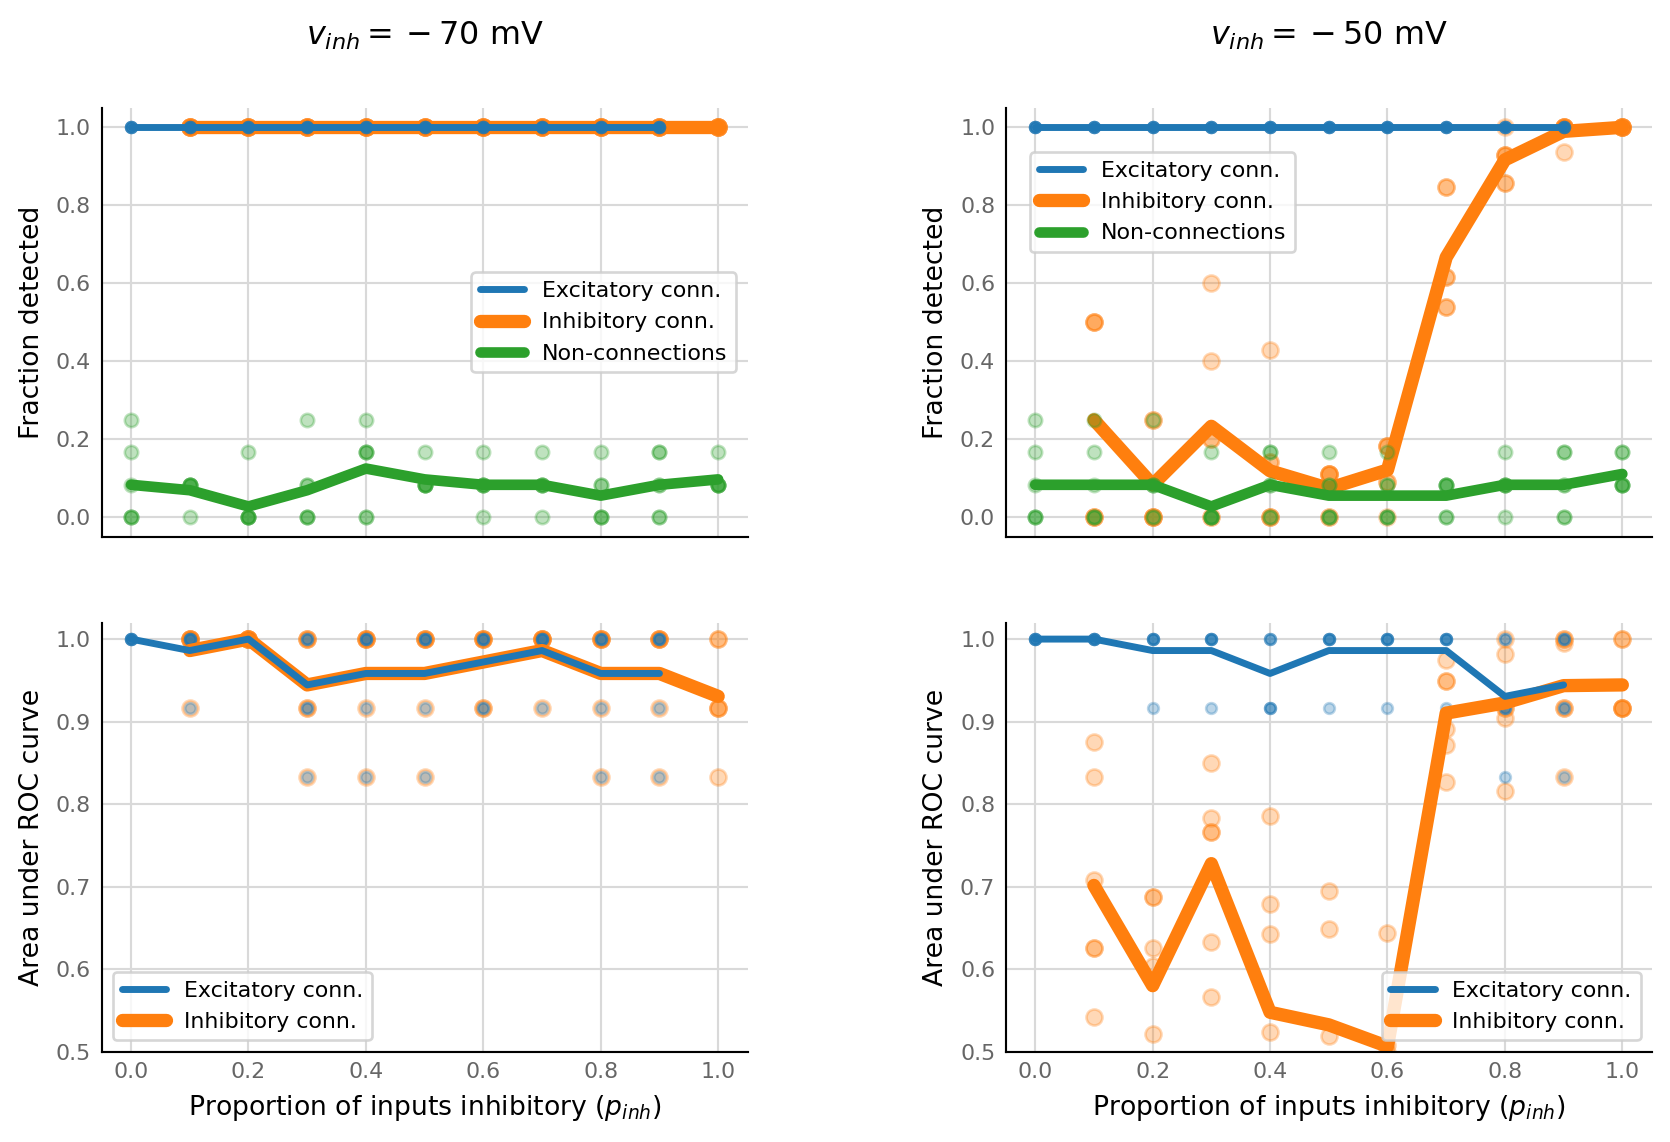
\includegraphics[w=1.47]{N_to_1_IE/performance_dots.png}
    }
  \captionn
  {STA detects inhibitory connections, but only when $\vinh < v_\text{rest}$ or when there are no excitatory inputs}
  {
    Connection detection performance of spike-triggered averaging at varying proportions of inhibitory inputs, and for two different inhibitory synaptic reversal potentials \vinh.
    \Top: Performance at a fixed detection threshold of $p < 0.05$ (where $p$ is the proportion of shuffled spike trains with an STA larger than the real spike train). Plotted are the true positive rates (separately for excitatory and inhibitory connections) and the false positive rate.
    \Bottom: Performance over all detection thresholds, as
    area under the ROC curve. As TPR is calculated separately for excitatory and inhibitory connections, there are also two ROC curves.
    For each condition, the simulation is run six times, each time with a different random number generator seed. The semi-transparent circles are individual simulations. The thick lines average over the seeds.\\
    Source: \nburl{2021-09-16__vary_E_vs_I}.
  }
  \label{fig:N_1_IE}
\end{figure}

\begin{figure}
    \hspace*{-2.5em}
    \subfloat{
        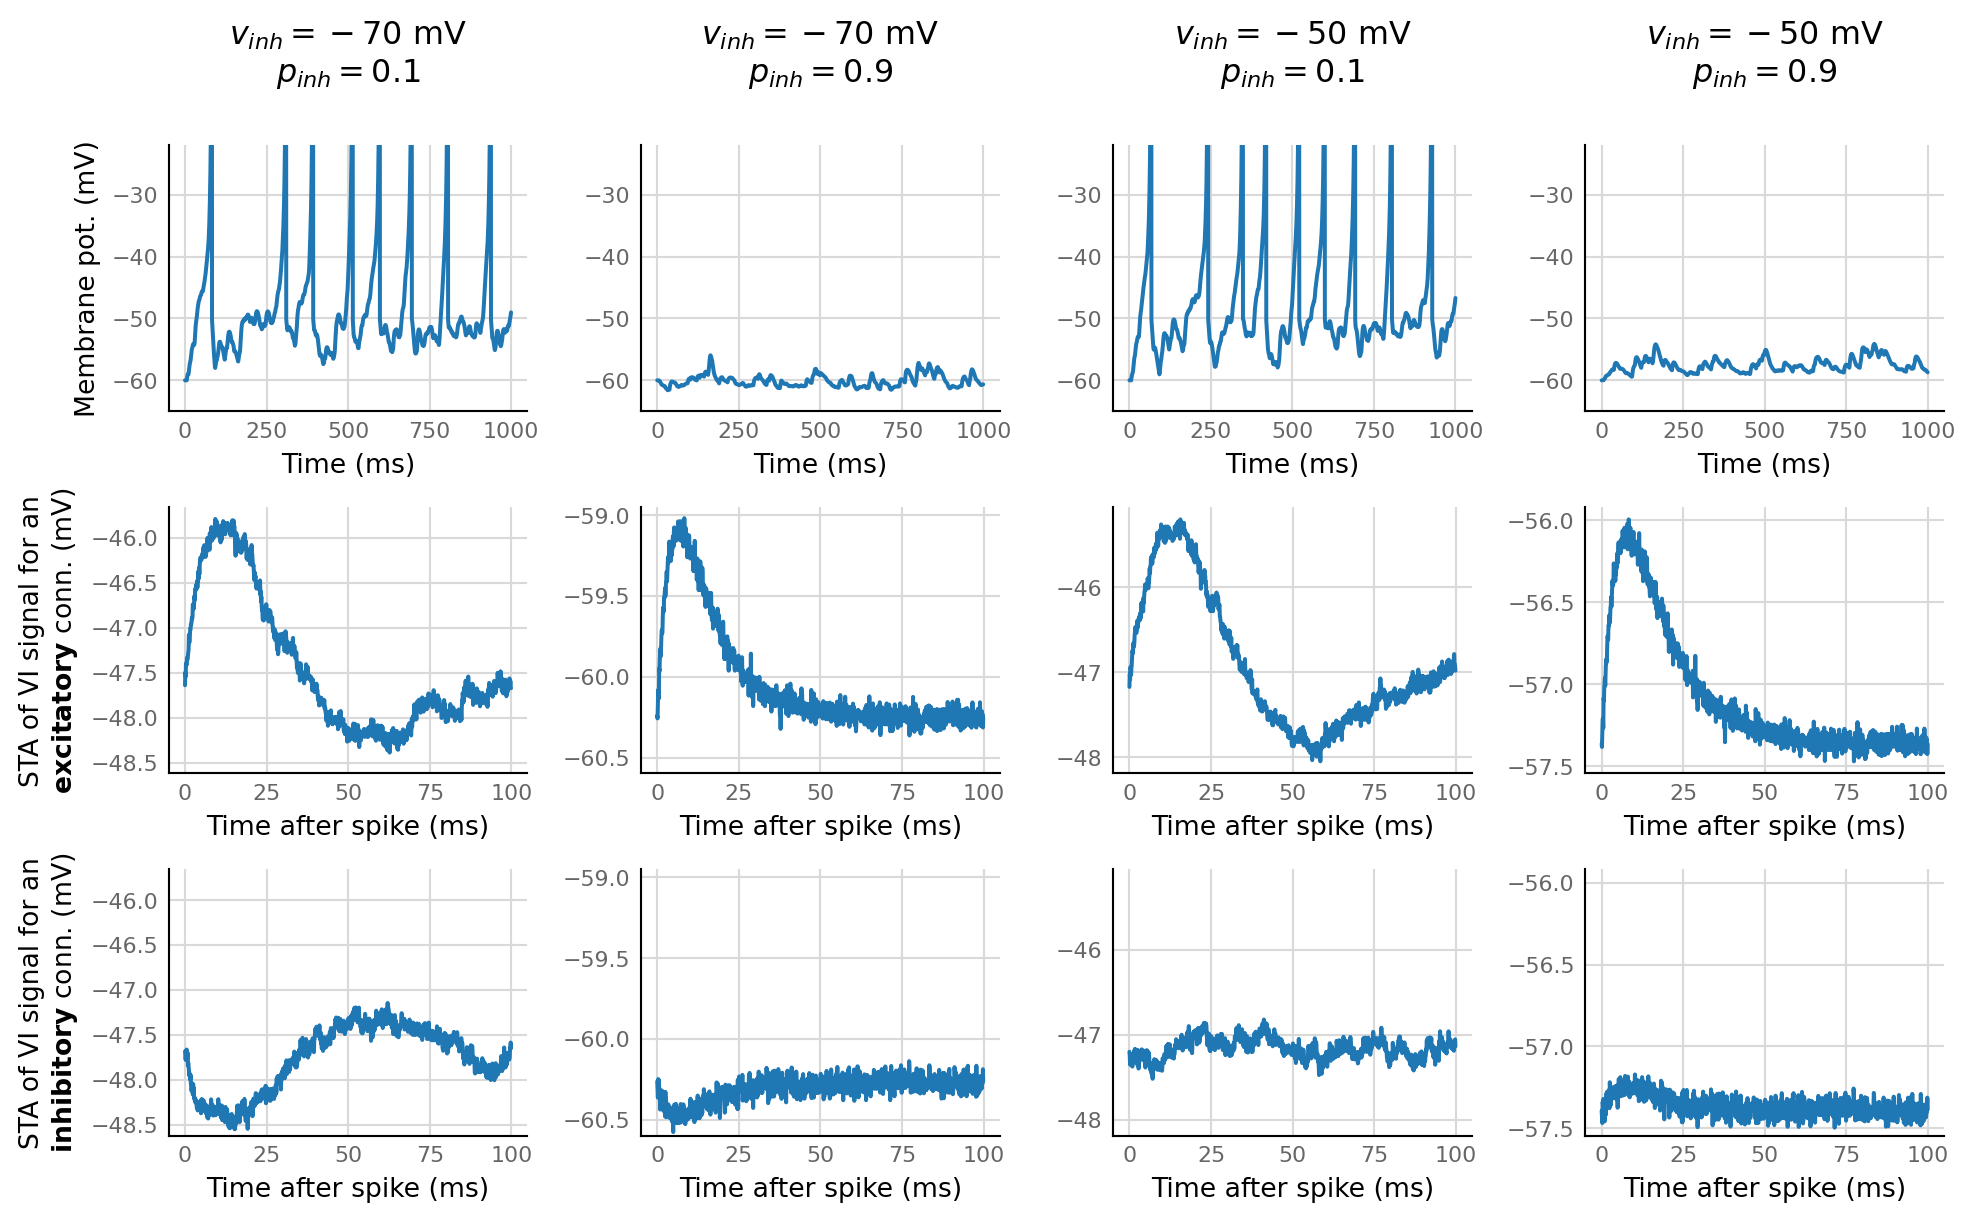
\includegraphics[w=1.58]{N_to_1_IE/inspect_signals.png}
    }
  \captionn
  {The inhibitory STA is flat when the reversal potential is close to the neuron's median voltage}
  {Excerpts from the Izhikevich simulation output (top row), and spike triggered averages of the voltage imaging signal (bottom two rows). The top voltage traces are shown without any VI noise for clarity. The actual STA's are in fact calculated on the noisy VI signal. Note that the y-axis extents of the STA's differ between columns (but are consistent within one).\\
  Source: \nburl{2021-09-16__vary_E_vs_I}.}
  \label{fig:N_1_signals}
\end{figure}


\subsection{Different synaptic conductances}

The synaptic conductance bump \dgsyn is now split into two different values: \dgexc and \dginh, for excitatory and inhibitory connections respectively.
\dgexc is fixed at $0.4$ nS. This value is chosen so that the output neuron has a realistic firing rate (less than one spike per second, but more than zero). \dginh is varied to be different multiples of this.

The ratio of inputs of either type is fixed at the physiological value of 4:1 excitatory:inhibitory, i.e. $\pinh = 0.2$. The fraction of connected inputs \pconn is set to $0.7$. All other simulation parameters stay the same.

We find that the STA method can detect connections when \dginh is at least as strong as \dgexc (\cref{fig:IE_ratio_perf}). This is straightforwardly explained by larger synaptic conductances causing larger PSP's, and thus larger STA's (\cref{fig:IE_ratio_signals}).

\begin{figure}
        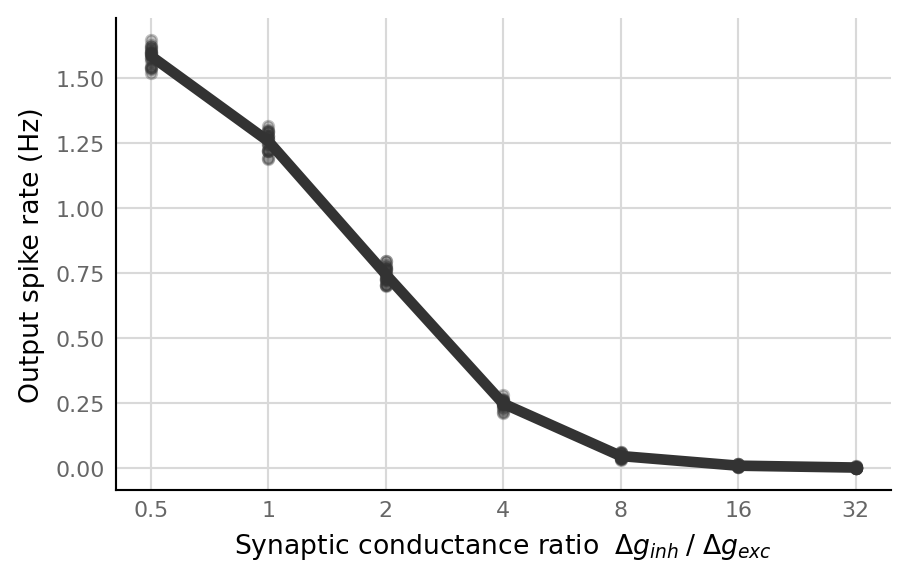
\includegraphics[w=0.8]{N_to_1_IE/ratio/spikes}\\[1em]
    \subfloat{
        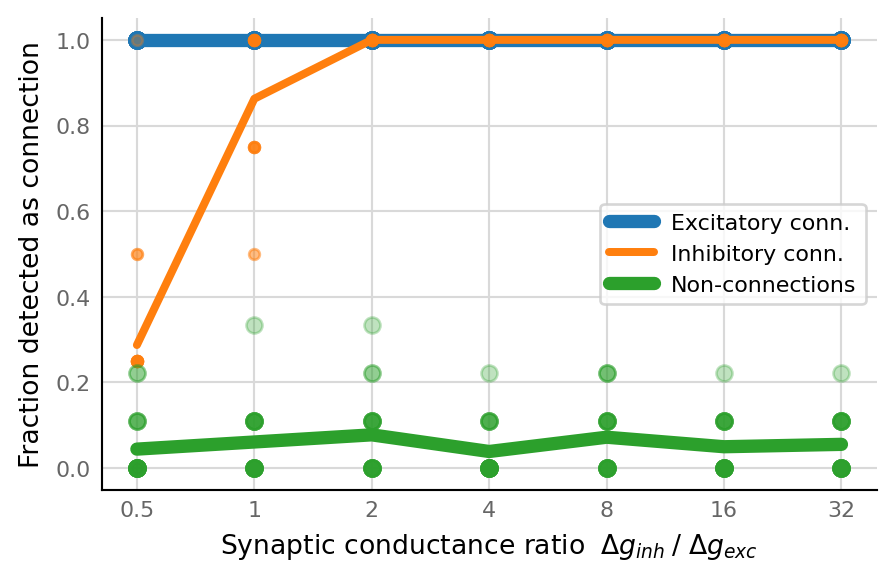
\includegraphics[w=0.8]{N_to_1_IE/ratio/rates}
        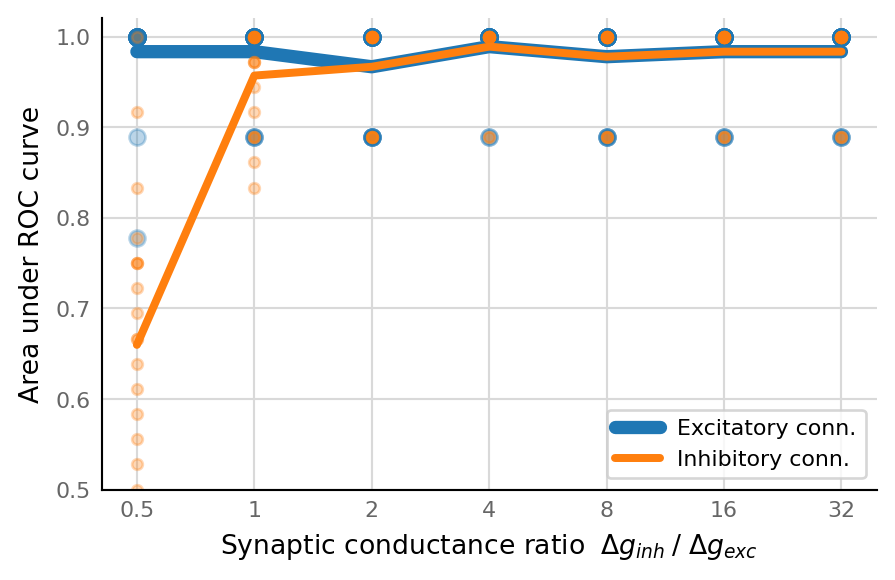
\includegraphics[w=0.8]{N_to_1_IE/ratio/aucs}
    }
    \captionn
        {STA detects inhibitory connections for most conductance ratios, and with or without output spikes}
        {Legend as in \cref{fig:N_1_IE}, but now with twenty simulations per condition, instead of six.
        Note that at a $p$-value threshold of $0.05$ (bottom left panel), we expect to see a false positive ratio of $0.05$, as can indeed be seen for most conductance ratios. With lower thresholds, we can decrease this FPR without decreasing recall, as evidenced by the AUC scores $\approx 1$.\\
        Source: \nburl{2021-11-05__vary_syncond_ratio}.
        }
  \label{fig:IE_ratio_perf}
\end{figure}

\begin{figure}
    \hspace*{-2.5em}
    \subfloat{
        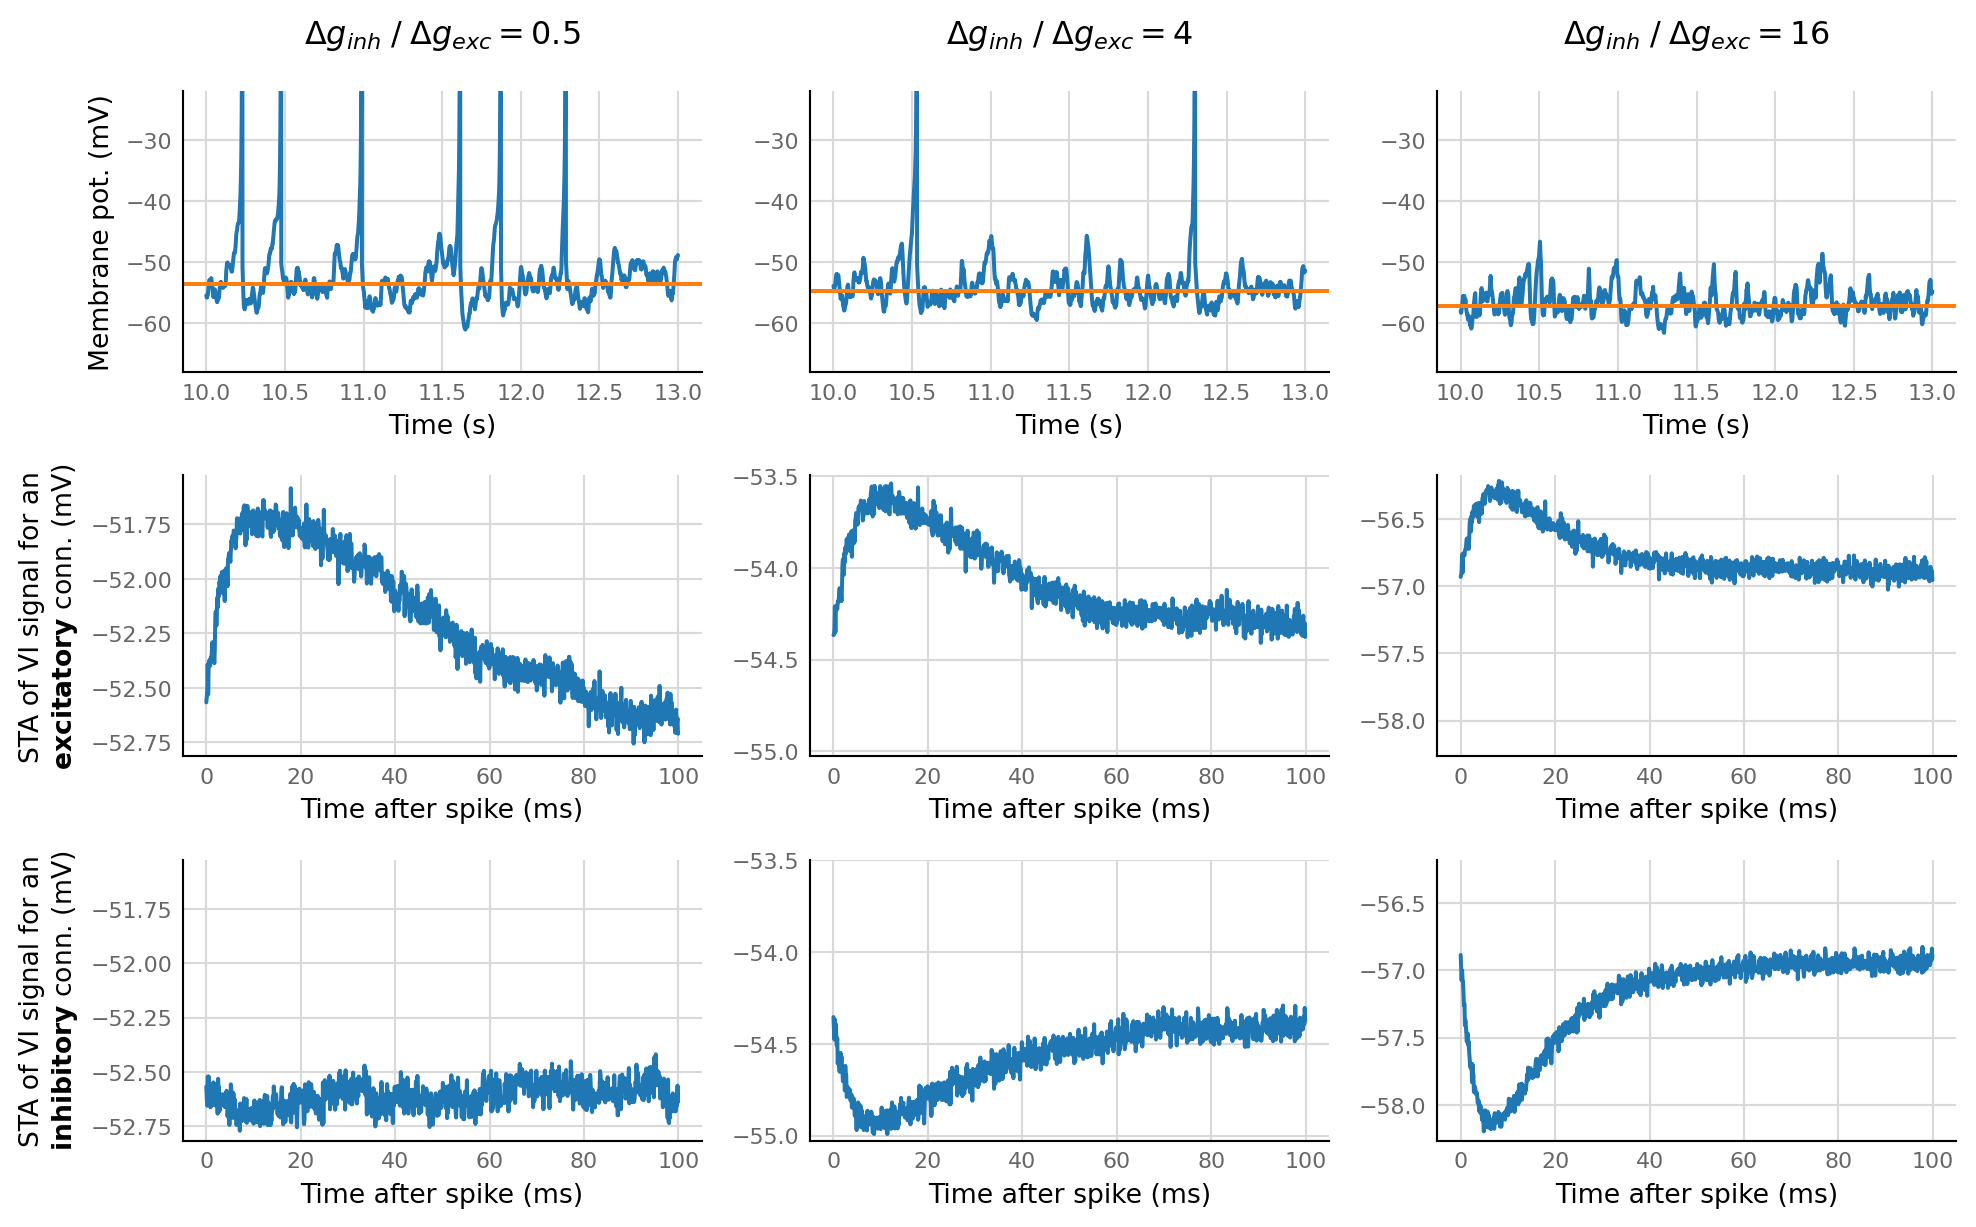
\includegraphics[w=1.6]{N_to_1_IE/ratio/signals}
    }
  \captionn
  {STA height increases with synaptic conductance}
  {Orange lines indicate the neuron's median voltage over the entire recording duration.\\
  Source: \nburl{2021-11-05__vary_syncond_ratio}.}
  \label{fig:IE_ratio_signals}
\end{figure}


\subsection{More connections versus stronger connections}

In the previous two subsections, we varied either the proportion of inhibitory inputs \pinh, or the inhibitory synaptic conductance \dginh.
Here, we vary both simultaneously.

We fix the number of excitatory inputs \Nexc to be $24$, and set the number of inhibitory inputs \Ninh to be a (sub)multiple of that. (Note that this changes the total number of inputs, which was fixed at $30$ up until now).
The synaptic conductance bump per excitatory spike \dgexc is fixed at $0.4$ nS as in the previous subsection, and \dginh is set to a multiple of that.

The multiples are chosen so that on the diagonal of \cref{fig:IE_tradeoff_grids}, the ratio of inputs is the inverse of the ratio of connection strengths: $\dginh / \dgexc = 4$ is matched with $\Ninh / \Nexc = 1 / 4$, etc.

We find that the spike triggered averaging method can detect both excitatory and inhibitory connections, over the entire parameter grid -- except, as found in the previous subsection, for weak inhibitory connections. In cortex, inhibitory connections are generally stronger than excitatory connections, so we should not find ourselves in this regime. Note also that we can detect incoming connections even when the neuron does not spike at all. This is a major advantage of voltage based connection detection versus spike-to-spike connection detection.

\begin{figure}
    \hspace*{-2.5em}
    \subfloat{
        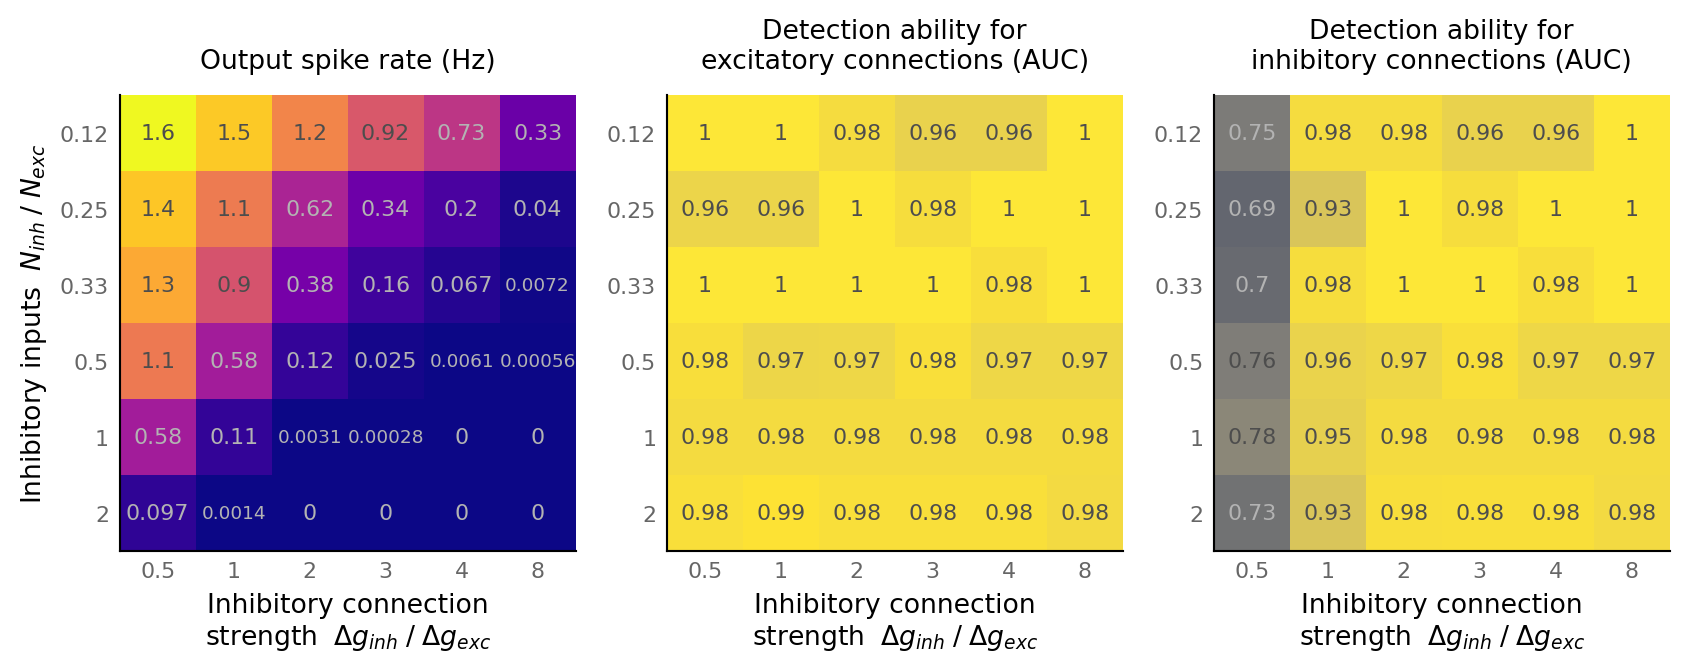
\includegraphics[w=1.6]{N_to_1_IE/tradeoff/grids.png}
    }
  \captionn
  {STA detects connections for weak or strong, sparse or dense inhibition}
  {Output firing rate (left) and connection detection performance (center and right) for different amounts and strengths of inhibitory inputs.
    Every cell is the mean of $6$ simulations.\\
    Source: \nburl{2021-11-11__vary_both_inh_strength_and_proportion}.}
  \label{fig:IE_tradeoff_grids}
\end{figure}

Focusing on the diagonal of \cref{fig:IE_tradeoff_grids} (highlighted in \cref{fig:IE_tradeoff_diag}), we notice that, notwithstanding the balancing, the firing rate increases for stronger but fewer connections. The reason is shown in \cref{fig:IE_tradeoff_sigs}: in these balanced regimes, the neuron can only fire when the inhibition is temporarily low enough for the excitation to overcome it, and make the neuron spike. When there are fewer inhibitory inputs, there will be more and longer such inhibition gaps (even though when there is inhibition, it is stronger, making the mean inhibition equal, as shown \cref{fig:IE_tradeoff_sigs} right).
This nonlinear phenomenon is typical in spiking simulations. In a mean-field model, where only firing \emph{rates} are simulated, this would not occur.

Looking at individual columns or rows of \cref{fig:IE_tradeoff_grids}, we find that the firing rate gently decreases above the diagonal, but below the diagonal it falls sharply to zero. This is again a consequence of simulating spikes: increasing the net excitation changes nothing about a zero firing rate, until the firing threshold is reached, above which net excitation and firing rate do change in lockstep.

Finally, we explain the high spread / multimodality in the firing rates of \cref{fig:IE_tradeoff_diag}. At the beginning of each simulation, when determining the number of input spike trains of each type (connected or not connected; excitatory or inhibitory), stochastic rounding is used. Say that there are $3$ inhibitory inputs (i.e. $1/8$th of the $24$ excitatory inputs, as on the far right of \cref{fig:IE_tradeoff_diag}). With our current connection probability \pconn of $0.7$, we should have $0.7 \times 3 = 2.1$ connected inhibitory inputs. With stochastic rounding, in $90\%$ of simulations there will be $2$ connected inhibitory inputs, and in $10\%$ of simulations there will be $3$. Those $10\%$ simulations with $3$ inhibitory connections are responsible for the cluster at the bottom right of the firing rate graph of \cref{fig:IE_tradeoff_diag}.

\begin{figure}
    \hspace*{-2.5em}
    \subfloat{
        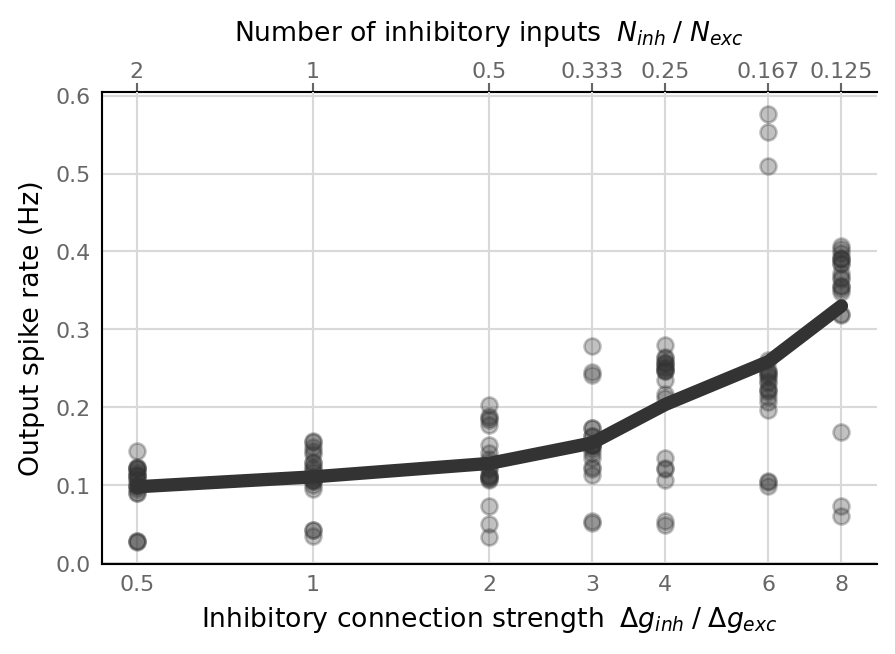
\includegraphics[w=0.78]{N_to_1_IE/tradeoff/diag_fr.png}
        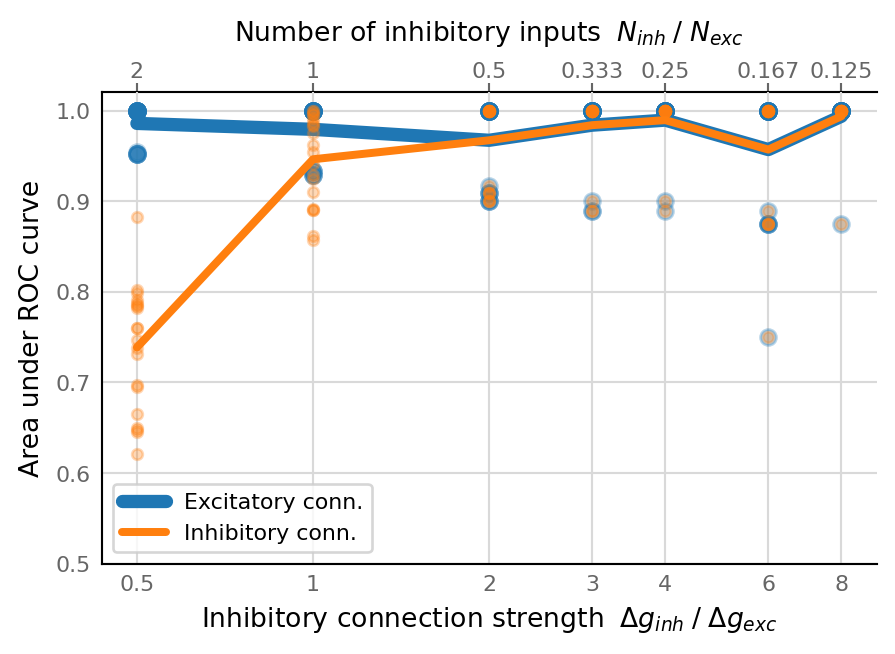
\includegraphics[w=0.78]{N_to_1_IE/tradeoff/diag_auc.png}
    }
  \captionn
  {Firing rate increases with stronger (but fewer) inhibitory inputs}
  {Excerpt of \cref{fig:IE_tradeoff_grids} along the diagonal (but with $20$ simulations per condition rather than $6$). Dots are individual simulations , lines are their means.\\
  Source: \nburl{2021-11-11__vary_both_inh_strength_and_proportion}.}
  \label{fig:IE_tradeoff_diag}
\end{figure}

\begin{figure}
    \hspace*{-2.5em}
    \subfloat{
        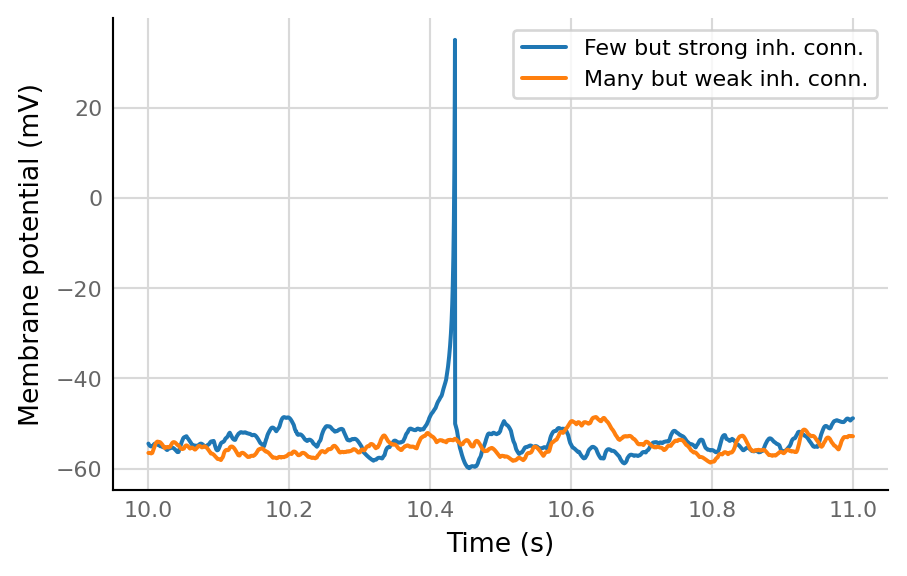
\includegraphics[w=0.78]{N_to_1_IE/tradeoff/sig_vm.png}
        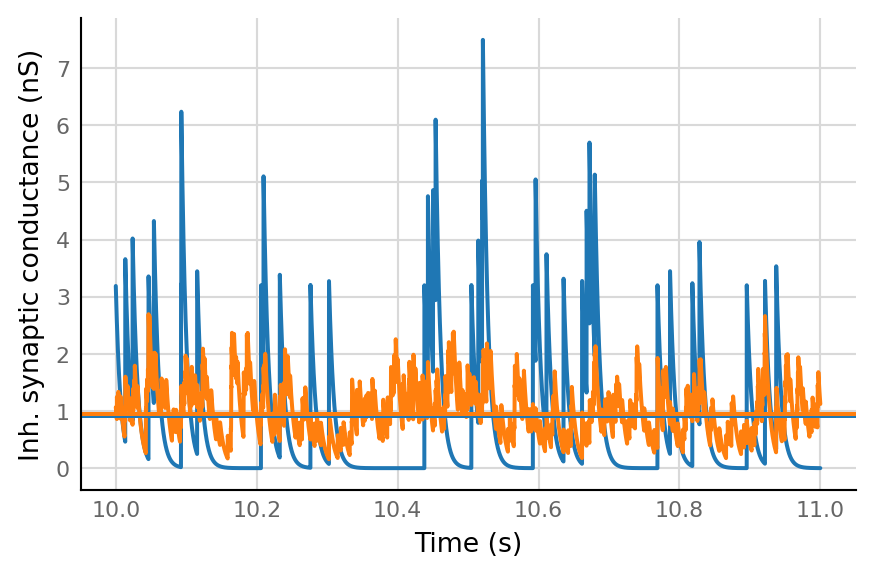
\includegraphics[w=0.78]{N_to_1_IE/tradeoff/sig_ginh.png}
    }
  \captionn
  {The neuron spikes during gaps in inhibitory input}
  {Excerpts from the membrane potential (left) and the total synaptic conductance of all inhibitory inputs (right) of two simulations. In the blue simulation, inhibitory inputs are $8$ times as strong as excitatory inputs, but there are $1/8$th times as many. In the orange simulation, the inhibitory inputs are as strong and as numerous as the excitatory inputs. Horizontal lines are means of the conductances over the entire simulation duration.
    Note the blue conductance gap around $t = 10.4$ seconds, allowing a spike.\\
    Source: \nburl{2021-11-11__vary_both_inh_strength_and_proportion}.}
  \label{fig:IE_tradeoff_sigs}
\end{figure}





\FloatBarrier
\section{Computational cost of STA test}

The brunt of the time in using the STA as a connection test is in actually calculating these STAs -- and the STAs of the shuffled versions of the tested spiketrains.

\Cref{tab:conntest-time-factors} lists different parameters that determine how long a connection test takes to run.

\begin{table}
    \begin{tabular}{l l l r l}
    Factor &               & Description                           & Value  & Unit            \\
    \toprule
    $ N_\mathrm{post} $&$ $& \makecell[l]{Number of analyzed voltage signals\\
        (number of postsynaptic neurons)}                          &$   1  $& voltage signals \\[0.8em]

    $ N_\mathrm{pre}  $&$ $& \makecell[l]{Number of tested spiketrains (possible\\
        presynaptic neurons) per `post' neuron }                   &$ 300  $& spiketrains     \\[0.8em]

    $ N_\mathrm{conn} $&$ = N_\mathrm{post} · N_\mathrm{pre} $&
        Number of connections tested                               &$ 300  $& connections     \\

    \midrule
    $ T   $&$             $& Duration of simulation or recording   &$  10  $& minutes         \\
    $ λ   $&$             $& Firing rate of presynaptic neuron     &$  16  $& spikes / second \\
    $ N_w $&$ = T · λ     $& Number of windows per tested conn.    &$ 9600 $& windows         \\
    \midrule
    $ T_w $&$             $& Window length                         &$  20  $& ms              \\
    $ Δt  $&$             $& Timestep of simulation or recording   &$  0.1 $& ms              \\
    $ f_s $&$ = 1 / Δt    $& Sample rate                           &$  10  $& samples / ms    \\
    $ M   $&$ = T_w · f_s $& Number of samples per window          &$  200 $& samples         \\
    \bottomrule
\end{tabular}

    \captionn{Factors in how long a connection test takes to run}
    {The listed values are ones typically used in this thesis.}
    \label{tab:conntest-time-factors}
\end{table}

% \begin{equation}
%     T = \mathrm{} · (1 + N_\mathrm{shuffled trains}) · λ · R
% \end{equation}
% with $λ$ the firing rate (spikes per second) of the presynaptic train

The chosen inputs to test (300 high firing trains) have a median firing rate of 16 Hz. I.e. at a simulation duration of 10 seconds, there are about 160 presynaptic spikes per tested connection. There are 101 times that many STAs to calculate per connection: once for the real spiketrain, and a 100 times for shuffles of it. For a 10 second simulation, there are thus about 16k STAs to calculate per connection.
For 10 minutes: 967k STAs. For 1 hour: 5.8M STAs.

The computation time of the STA-based test thus scales linearly with the voltage imaging recording duration. We find that testing 300 possible spiketrain inputs to one neuron takes about one-fifth of the time of the recording (\cref{fig:STA_compute_time}): about 2 minutes of computation time for a 10-minute recording.

\begin{figure}
    \begin{sidecaption}
        {\textbf{Test time scales linearly with voltage signal duration}.\\
        Simulation timestep ('sample time') of 0.1 ms. STA length of 20 ms; i.e. 200 samples.\\
        Black dots are the means over five simulations per duration. Compute times for individual simulations are plotted with gray dots; but the variation is so small that these gray dots are hidden behind the black means. Gray dashed line is the $y = x$ identity.  Source: \nburl{2023-09-20__STA_conntest_for_diff_recording_quality_n_durations}.}
        [fig:STA_compute_time]
        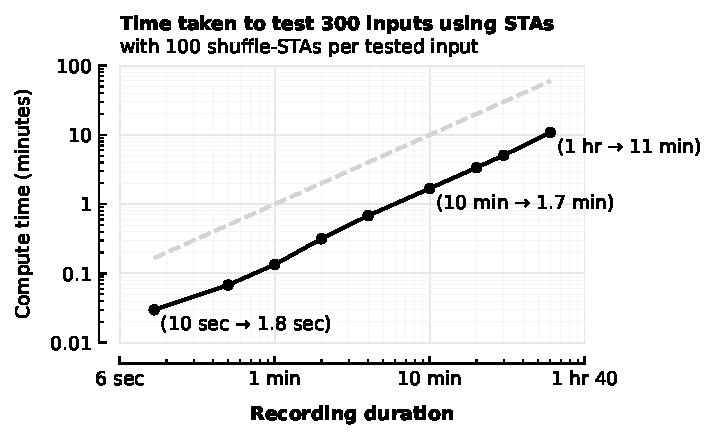
\includegraphics{STA_compute_time}
    \end{sidecaption}
\end{figure}


\FloatBarrier
\section{Conclusion}

Using spike-triggered-averages of the postsynaptic voltage is an obvious way to look for post-synaptic potential bumps, and to thus detect neuron connections.

In this chapter we have found that this STA method indeed does significantly better than chance at detecting conections, under realistic conditions (6500 EI-balanced inputs to one neuron, 10-minute recording, voltage imagaing SNR of 40).
Of the highest firing inputs (100 excitatory, 100 inhibitory), we detect about 65\%, at a precision level where 65\% of our detections are correct. The AUC is about $0.50$.

% better: TPR at FPR of 0.05 (e.g.). But need to re-run nb.
% (the sweeps are on disk :)).

This is significantly better than chance (AUC at chance level is $0.252$), but there is a lot of room for improvement. In a later chapter (\cref{ch5-new-methods}), we will look for improved connection detection methods. But first, we take another look at our test setup.

In this chapter, only one neuron's voltage was simulated, while being stimulated by $N$ independent Poisson spiketrains. Real neural networks are often more recurrent and less feedforward than this, and different inputs to the same neuron can be correlated. This is why, in the next chapter, we simulate the voltages of multiple neurons, connected to each other in a fully recurrent neural network. In particular, we want to test the problem of indirect connections that are detected as direct connections -- a well-known problem in the spike-to-spike connection inference literature.\cite{Orlandi2017FirstConnectomicsChallenge,Das2020SystematicErrorsConnectivity}
